\documentclass[preprint]{sigplanconf}
\usepackage{amssymb}
\usepackage{graphicx}
\usepackage{amsmath}
\usepackage{mathptmx}
\usepackage{hyperref}
\usepackage{alltt}
\usepackage{url}
\usepackage{float}
\usepackage{style/utils}
\usepackage{style/code}
\usepackage{style/proof}

% -----------------------------------------------------------------------------
\begin{document}

\title{Fusing Filters with Integer Linear Programming}
% Better title?
% \title{Better fusion for filters}

\authorinfo{ 
  Amos Robinson$^\dagger$ 
  \and Ben Lippmeier$^\dagger$
  \and Manuel M. T. Chakravarty$^\dagger$
  \and Gabriele Keller$^\dagger$ 
}{
  \vspace{5pt}
  \shortstack{
    $^\dagger$Computer Science and Engineering \\
    University of New South Wales, Australia \\[2pt]
    \textsf{\{amosr,benl,chak,keller\}@cse.unsw.edu.au}
  }
}

\maketitle
\makeatactive

\begin{abstract}
Recent work on array fusion shows how to extract data-flow graphs from functional programs and compile them into efficient imperative loops. However, the compilation process only handles graphs that can be compiled into \emph{single} loops, and most programs require more. Prior work shows how use Integer Linear Programming (ILP) to \emph{cluster} the operators in a general data-flow graph into subgraphs that can be individually fused, but until now this approach did not handle filter-like operators which produce arrays of a different size than the input. We extend the existing ILP approach with support for filters, using an external ILP solver to find good clusterings.
\end{abstract}


\category
	{D.3.3}
	{Programming Languages}
	{Language Constructs and Features---Concurrent programming structures; Control structures; Abstract data types}

\terms
	Languages, Performance

\keywords
	Arrays, Fusion, Haskell

%!TEX root = ../Main.tex
\section{Introduction}

Data flow fusion~\cite{lippmeier2013flow} is a technique to compile a specific class of data flow programs into single, efficient imperative loops. This process of ``compilation'' is equivalent to performing array fusion on a combinator based functional array program, as per related work on stream fusion~\cite{coutts2007streamfusion} and delayed arrays~\cite{keller2010repa}. The key benefits of data flow fusion over this prior work are: 1) it fuses programs that use branching data flows where a produced array is consumed by several consumers, and 2) complete fusion into a single loop is guaranteed for all programs that operate on the same size input data, and contain no fusion-preventing dependencies between operators.

Fusion-preventing dependencies express the fact that some operators simply must wait for others to complete before they can produce their own output. For example, in the following:
\begin{code}
  normalize :: Array Int -> Array Int
  normalize xs = let sum = fold (+) 0 xs
                 in  map (/ sum) xs
\end{code}

If we wish to divide every element of an array by the sum of all elements, then it seems we are forever destined to compute the result using at least two loops: one to determine the sum, and one to divide the elements. The evaluation of @fold@ demands all elements of its source array, and we cannot produce any elements of the result array until we know the value of @sum@. 

However, many programs \emph{do} contain opportunities for fusion, if we only knew which opportunities to take. The following example offers \emph{several} unique, but mutually exclusive approaches to fusion. Figure~\ref{f:normalize2-cluterings} on the next page shows some of the possibilities.
\begin{code}
 normalize2 :: Array Int -> Array Int
 normalize2 xs
  = let sum1 = fold   (+)  0   xs
        gts  = filter (> 0)    xs
        sum2 = fold   (+)  0   gts
        ys1  = map    (/ sum1) xs
        ys2  = map    (/ sum2) xs
    in (ys1, ys2)
\end{code}

In Figure~\ref{f:normalize2-cluterings}, the dotted lines show possible clusterings of operators. Stream fusion implicitly choses the solution on the left as its compilation process cannot fuse a produced array into multiple consumers. The best existing ILP approach will chose the solution on the right as it cannot cluster operators that consume arrays of different lengths. Our system choses the solution in the middle, which is also optimal for this example. 

% NOTE: This set of bullets needs to fit on the first page, without spilling to the second.
Our contributions are as follows:
\begin{itemize}
\item   
We extend prior work by Megiddo~\cite{megiddo1998optimal} and Darte~\cite{darte2002contraction}, with support for length changing operators. Length changing operators can be clustered with the operators that generate their source arrays, and compiled naturally with data-flow fusion (\S\ref{s:ILP}).

\item
We present a simplification to constraint generation that is also applicable to some existing integer linear programming formulations such as Megiddo's,
where constraints between two nodes need not be generated if there exists a fusion-preventing path between the two (\S\ref{s:OptimisedConstraints}).

\item
Our constraint system also encodes a total ordering on the cost of clusterings, expressed using weights on the integer linear program. For example, we encode that memory traffic is more expensive than loop overheads, so given a choice between the two, the memory traffic will be reduced (\S\ref{s:ObjectiveFunction}).

\item
We present benchmarks of our algorithm applied to several common programming patterns, and to several pathological examples.
Our algorithm is complete and yields good results in practice, though if array sizes are unknown, an optimal solution is uncomputable in general. \TODO{ref}
\end{itemize}

The reduction of the clustering problem to integer linear programming was previously described by~\cite{megiddo1998optimal}, though they do not consider length changing operators.


% We must also decide which clustering is the `best' or most optimal. One obvious criterion for this is the minimum number of loops, but there may even be multiple clusterings with the minimum number of loops. In this case, the number of required manifest arrays must also be taken into account. 

% As real programs contain tens or hundreds of individual operators, performing an exhaustive search for an optimal clustering is not feasible, and greedy algorithms tend to produce poor solutions. 


\section{Combinator normal form}
We can accept functions written in \emph{combinator normal form}, which is a specialised form of first-order array programs detailed in Figure~\ref{f:CombinatorNormalForm}.
This form is a list of combinator bindings, where variables are split into scalar and array variables.
The main restriction is that worker functions may only reference scalar variables, and thus do not perform array combinators.

The only combinators we fuse are @map@, @filter@, @fold@ and @gather@.
Most of these are standard combinators except for @gather@, which is equivalent to @gather xs ys = map (index xs) ys@.
However, as we support no @index@ operation, @gather@ is implemented as a primitive.

Since it is unlikely that an entire function will be comprised of these few combinators, we support one additional binding type: @external@. This signifies that the referenced variables are used by a computation that is not a primitive combinator, and must be materialised fully in memory at this stage.
The @external@ also signifies variables produced by a non-primitive combinators.
Without knowing the nature of the computation expressed by @external@, we must naturally take a conservative view, and allow no fusion to occur between at these points. They are, in effect, fusion barriers, forcing arrays and scalars to be fully computed before continuing.

It is important to note that because of the purity of Haskell, we are free to take certain liberties when reordering the program.
None of the worker functions, nor any @external@ computations may produce visible side-effects; the only observable effect must be to produce their output.
%!TEX root = ../Main.tex
\begin{figure}
\begin{tabbing}
MMMM        \= MM \= MMMMMMMMM \= \kill
$scalar$    \> $\to$ \> (scalar variable) \\
$array$     \> $\to$ \> (array variable)  \\
$f$         \> $\to$ \> (worker function) \\
$fun$       \> $\to$ \> $f~scalar\ldots$
\\[2ex]
$bind$      \> @::=@ \> $scalar$ \> $=~sbind$ \\
            \> $~|$  \> $array$  \> $=~abind$ \\
            \> $~|$  \> $scalar\ldots,array\ldots$ \> $=~@external@~scalar\ldots~array\ldots$
\end{tabbing}

\begin{tabbing}
MMMM        \= MM \= MMMMM \= MMMMMM \= M \= MMMM \= MMMMMM \= \kill
$sbind$     \> @::=@ \> $@fold@$     \> $fun~~ array$
\\[1ex]

$abind$     \> @::=@ \> $@map@_n$    \> $fun~~ array^n$ 
            \> $~|$  \> $@filter@$   \> $fun~~ array$   \\
            \> $~|$  \> $@generate@$ \> $scalar~~ fun$  
            \> $~|$  \> $@gather@$   \> $array~~ array$ \\
            \> $~|$  \> $@cross@$    \> $array~~ array$
\\[1ex]
$function$  \> @::=@ \> $\lambda scalar\ldots~array\ldots~\to$ \\
            \>          \> $@let@~bind\ldots$                  \\
            \>          \> $@in@~(scalar\ldots,~array\ldots)$
\\[3ex]
$@fold@$     \> $:~ (a \to a \to a) \to @Array@~~ a \to a$     \\
$@map@_n$    \> $:~ (\{a_i          \to\}^{\;i\; \gets 1 \dots n}~~ b)  \to
                       \{@Array@~~ a_i \to\}^{\;i\; \gets 1 \dots n}~~ @Array@~~ b$ \\
$@filter@$   \> $:~ (a \to @Bool@) \to @Array@~~ a \to @Array@~~ a$      \\
$@generate@$ \> ~~ $:~ @Nat@ \to (@Nat@ \to a) \to @Array@~~ a$          \\
$@gather@$   \> ~~ $:~ @Array@~~ a \to @Array@~~ @Nat@  \to @Array@~~ a$ \\
$@cross@$    \> ~~ $:~ @Array@~~ a \to @Array@~~ a ~~~~ \to @Array@~~ a$
\end{tabbing}
\caption{Combinator normal form}
\label{f:CombinatorNormalForm}
\end{figure}





%!TEX root = ../Main.tex
\section{Size inference}

Knowing the relative sizes of loops is important for fusion.
While it \emph{is} technically possible to fuse loops of different sizes, it requires extra complexity to find the maximum of the loop sizes, and additional branches are required to only execute the smaller loop fewer times. For simplicity, we do away with this added complexity and only support fusion of equal sized loops. \emph{Size inference} is performed on the combinators to infer as much information as possible about the sizes of the resulting loops.

It is important to emphasise that we are only interested in relative sizes of arrays; which arrays are equal, and which may be smaller.
The $@map@_n$ combinators require all input arrays to be the same size, and their output is the same.
Since @fold@s do not produce arrays, they have no constraints.
@gather@ takes two arrays; the data and the indices. Its output size is the size of the indices.
The size of a @filter@'s output is most interesting; the exact size is not known until after it has been executed, only that it is less than or equal to the input size.
Similarly, the size of @external@ outputs is not known at all, and thus cannot be constrained.

Size inference has been explored before in the context of fusion by Chatterjee~\cite{chatterjee1991size}, but the only constraints they support are equality.
Their formulation has no filtering operations, and all array operations in their case generate the same size as at least one of the operation's inputs.
A more in-depth analysis has also been explored by Jay~\cite{jay1996shape} in the form of shape inference, which is built from primitives such as @cons@ and @nil@.
Since we have fewer primitives and simpler goals, our size inference does not need to be as complicated as Jay's shape inference.


Our formulation of size inference is very similar to type inference, a la \CITE.
First, constraints are generated for the bindings, such as equality among two rates, the conjunction of two constraints, and existentials.
If these constraints can be solved, the equality constraints are used to group the rates into equivalence classes.
Otherwise if the constraints are unable to be solved, the program cannot be assured to require no runtime size checks and will not be fused by our system.
After the constraints are generated and solved, each combinator is given an iteration size.
Two loops with the same iteration size can be fused together.

\newcommand{\constr}[1]{\llbracket #1 \rrbracket}
\newcommand{\hole}[0]{[]}
\newcommand{\fillhole}[2]{#1\left[#2\right]}

\subsection{Constraint generation}
Rates may either be some rate variable, $k_n$ where $n$ is the name of an array, or they may be a cross product of two rates.

\begin{tabbing}
MMMMM       \= MM \= MMMMMMMMMMM \= \kill
$rate$      \> @::=@ \> $k_n$               \> (rate variable)\\
            \> $~|$  \> $rate \times rate$  \> (cross product) \\
%            \> $~|$  \> $Filtered_n$        \> (output of @filter@s) \\
%            \> $~|$  \> $External_n$        \> (output of @external@s) \\
\end{tabbing}

The most important constraint is equality on two rates.
Context holes are used to simplify later definitions, and the notation $\fillhole{c}{d}$ is used to denote replacing all holes in $c$ with $d$.
Constraints may be joined together with $c \wedge d$, which requires both $c$ and $d$ to be satisfiable.
Forall quantifiers may be given an upper bound, and mean the constraint must be satisfiable for every rate.
Existential quantifiers simply state that there must exist a rate that satisfies the constraint.


\begin{tabbing}
MMMMM       \= MM \= MMMMMMMMMMM \= \kill
$C$          \> @::=@ \> $true$                                 \> (trivially true) \\
             \> $~|$  \> $\hole$                                \> (constraint hole) \\
             \> $~|$  \> $rate = rate$                          \> (equality constraint) \\
             \> $~|$  \> $C \wedge C$                           \> (conjunction) \\
             \> $~|$  \> $\forall k_n.\ C$                      \> (forall quantification) \\
             \> $~|$  \> $\exists k_n.\ C$                      \> (existential quantification)\\
%             \> $~|$  \> $\exists k_n \le rate.\ C$             \> (exists with upper bound)    \\
\end{tabbing}


Constraints are generated for a list of bindings.
As folds produce no constraints, they simply return a hole to be filled later.
Maps require their inputs and output to all have the same rate, so if there exists some rate that is equal to all its inputs, then that is the rate of the output.
As the output rate of a filter is unknown and cannot be constrained except for the upper bound, it is a forall: for all possible rates, the subconstraint must be satisfiable.
Similarly, external must work for any possible output, so the subconstraint must be satisfiable for all rates.

The final clauses show how the constraint holes are filled by constraints of subsequent bindings.
If there no bindings, the constraint is trivially true.

$$\begin{array}{lcrcl}
&&\constr{\_} & :: & binds \rightarrow C \\
\\
% MMMMMMMMMMMMMMMMMM \= MM \= \kill
% $\constr{\lambda scalars~arrays \to @let @binds@ in @x}$ \> $=$ \> $\forall_{a \in arrays} k_a. \constr{binds}$ \\

\constr{o &=& @fold @f@ @n}       &  = &  \hole \\
\constr{o &=& @map@_n~f~ns}       &  = &  \exists k_o.\ \bigwedge_{n \in ns}\{k_o = k_n\} \wedge \hole \\
\constr{o &=& @filter@~f~n}       &  = &  \forall k_o.\ \hole \\
\constr{o &=& @gather@~i~d}       &  = &  \exists k_o.\ k_o = k_i \wedge \hole \\
\constr{o &=& @cross@~a~b}        &  = &  \exists k_o.\ k_o = k_a \times k_b \wedge \hole \\
\constr{outs &=& @external@~ins}  &  = &  \forall_{o \in outs} k_o.\ \hole \\
\\
&&\constr{b;~bs}  &  = &  \fillhole{\constr{b}}{\constr{bs}}       \\
&&\constr{nil}    &  = &  true                          \\
\end{array}$$

\subsubsection{Examples}

As an example of constraint generation, here is the @normalize2@ program from earlier.
\begin{tabbing}
@MMMMMMMMMMMMMMMMMMMMMMMMMMMMMMMM@  \= \kill
@normalize2 us@                     \> $\exists k_{us}.$      \\
@ = let sum1 = fold   (+) 0 us@     \>                      \\
@       gts  = filter (>0)  us@     \> $\forall k_{gts}.$ \\
@       sum2 = fold   (+) 0 gts@    \> \\
@       nor1 = map  (/sum1) us@     \> $\exists k_{nor1}.\ k_{nor1} = k_{us} \wedge$ \\
@       nor2 = map  (/sum2) us@     \> $\exists k_{nor2}.\ k_{nor2} = k_{us} \wedge$ \\
@   in (nor1, nor2)@                \> $true$ \\
\end{tabbing}
This constraint is satisfiable, with the equivalence classes being:
\newcommand{\eqclasses}[1]{
    \begin{tabbing}
        MM \= M \= \kill
        #1
    \end{tabbing}}
\newcommand{\eqclass}[2]{$#1$ \> $\in$ \> $\{#2\}$ \\}
\eqclasses{
    \eqclass{k_{us}}{k_{us}, k_{nor1}, k_{nor2}}
    \eqclass{k_{gts}}{k_{gts}}
}

The next example involves two filters using the same predicate.
Despite using the same predicate and input data, we produce different output rates for each filter.
\begin{tabbing}
@MMMMMMMMMMMMMMMMMMMMMMMMMMMMMMMM@  \= \kill
@diff xs@                           \> $\exists k_{xs}.$ \\
@ = let ys1 = filter p xs@          \> $\forall k_{ys1}.$       \\
@       ys2 = filter p xs@          \> $\forall k_{ys2}.$       \\
@   in (ys1, ys2)@                  \> $true$                   \\
\end{tabbing}

This constraint is satisfiable, with the equivalence classes being:
\eqclasses{
    \eqclass{k_{xs}}    {k_{xs}}
    \eqclass{k_{ys1}}   {k_{ys1}}
    \eqclass{k_{ys2}}   {k_{ys2}}
}

This example is disallowed, as it would require a runtime check on the size of the @flt@ array.
\begin{tabbing}
@MMMMMMMMMMMMMMMMMMMMMMMMMMMMMMMM@  \= \kill
@bad1 vs@                           \> $\exists k_{vs}.$ \\
@ = let flt   = filter p vs@        \> $\forall k_{flt}.$ \\
@       wrong = map2   f flt vs@    \> $\exists k_{wrong}.\ k_{wrong} = k_{flt}$ \\
                                    \> $\wedge k_{wrong} = k_{vs} \wedge$ \\
@   in  wrong@                      \> $true$
\end{tabbing}
This constraint is unsatisfiable, as by transitivity it can be simplified to $\exists k_{vs}.\ \forall k_{flt}.\ k_{vs} = k_{flt}$.
Obviously, there exists no sole size such that all sizes are equal to it.
As a result, no equivalence classes are generated for this example, and no fusion is performed.


Similarly, this example is not allowed, as it would require a runtime check to determine that the output of two filters @flt@ and @flt2@ are the same size.
\begin{tabbing}
@MMMMMMMMMMMMMMMMMMMMMMMMMMMMMMMM@  \= \kill
@bad2 vs@                           \> $\exists k_{vs}.$ \\
@ = let flt  = filter p  vs@        \> $\forall k_{flt}.$ \\
@       flt2 = filter p' vs@        \> $\forall k_{flt2}.$ \\
@       mix  = map2   f  flt flt2@  \> $\exists k_{mix}.\ k_{mix} = k_{flt}$ \\
                                    \> $\wedge k_{mix} = k_{flt2} \wedge$ \\
@   in  mix@                        \> $true$                               \\
\end{tabbing}
Again, by transitivity of equality this constraint can be simplified to $\forall k_{flt}.\ \forall k_{flt2}.\ k_{flt} = k_{flt2}$.
It is easy to see that this constraint is unsatisfiable.


\subsection{Iteration size}
After the constraints are solved, each combinator is assigned a $rate$ as an iteration size -- the size of the loop required to generate the output.
It is important to note that for filters, the iteration size is not the output size, but is instead the size of the input.
The output size of a filter is, however, a \emph{subsize} of the input's size, as not only is it known to be less than or equal to its input in size, it is also generated depending on the input.
The iteration sizes, $\tau_n$, are used to check whether two loops may be fused.
Any two iteration sizes in the same equivalence class are the same size, and so are fusible.
The difference from previous work is that loops of different iteration sizes \emph{can} be fused, if one is a subsize of the other, and the subsize's \emph{generator} is fused together it as well.
Basically, operations on filtered data can be fused with operations on the original data, if it is fused with the filter as well.
External computations are treated separately, as they cannot be fused with any other nodes.

\begin{tabbing}
MMMMM       \= MM \= MMMMMMMMMMM \= \kill
$\tau$       \> @::=@ \> $rate$                                  \> (loop size of some rate) \\
             \> $~|$  \> @external@                              \> (external and unfusible) \\
\end{tabbing}

Once the constraints are solved, known to be satisfiable, and sorted into equivalence classes, each combinator is assigned a rate.
Note that for a filter, the size of the output array $k_o$ is some existential that is less than or equal to $k_n$, but the actual loop size of the \emph{combinator} is equal to $k_n$.
This is because, in order to produce the filtered output, all elements of the input $n$ must be considered.


\begin{tabbing}
MM \= MM \= MMMMMMMMM \= MMMM \= MM \= \kill
$\tau$  \>$::$\> $binds \rightarrow name \rightarrow \tau$ \\
\\
$\tau_{bs,o}$    
            \> $|$ \> $o = @fold@~f~n$      \> $\in bs$ \> $=$ \> $k_n$ \\
            \> $|$ \> $o = @map@_n~f~ns$    \> $\in bs$ \> $=$ \> $k_o$ \\
            \> $|$ \> $o = @filter@~f~n$    \> $\in bs$ \> $=$ \> $k_n$ \\
            \> $|$ \> $o = @gather@~i~d$    \> $\in bs$ \> $=$ \> $k_i$ \\
            \> $|$ \> $o = @cross@~a~b$     \> $\in bs$ \> $=$ \> $k_a \times k_b$ \\
            \> $|$ \> $o = @external@~ins$  \> $\in bs$ \> $=$ \> $@external@$ \\
\end{tabbing}

Solving the generated equality constraints allows each rate to be grouped into equivalence classes.
All combinators whose constraints are in the same equivalence class have the same iteration size, and may be fused together.
These constraints are also used to rule out any programs that require runtime checks on array lengths during the program.

\subsection{Runtime checks on array lengths}
The $@map@_n$ combinator requires all its input arrays to be the same size.
We do not, however, want to perform runtime checks on the size of arrays before every combinator.
We have decided to only fuse programs that can be statically determined to require only array length checks at the start of execution. 

\TODO{We assign different rates to both @ys1@ and @ys2@ in this example.}
\begin{code}
 diff xs = let ys1 = filter p xs
               ys2 = filter p xs
           in  (ys1, ys2)
\end{code}


% \ben{This point is only relavant in the context of our specific implementation, which is no the focus of this paper. }
% Any other programs are simply left alone by our fusion system, potentially falling back to stream fusion.


We use the constraints to rule out any programs that require runtime checks on array lengths during the program. Firstly, filter and external constraints are only allowed to be mentioned after their binding site, as it is only at that stage that the lengths are actually known.

\ben{Refactor presentation to use the actual $\exists k. $ quantifier, as in ``The essence of ML type inference'', from ATAPL}

Secondly, it is not possible to constrain one constructor to equal another: $Filtered_n = External_n$ is invalid. Finally, any initial equality constraints, such as two input arrays being the same length, or one input array being the length of the cross product of two others, are dealt with by inserting runtime checks only at the start of the function.


The constraints $Filtered_n$, $External_n$ are treated as \emph{existential} constructors, bound at $n$. This means that such constraints are not able to be referred to before their bindings.
Intuitively, we know that the output of a @filter@ or an @external@ has \emph{some} length, but we don't know what its value is until after they have executed. Thus, constraining the input of something to be some exact length, before we know what the length is, is impossible.

Similarly, these constructors cannot be constrained to equal any other constructor. 
For example, $Filtered_n = External_n$ is invalid, as is $a \times b = Filtered_n$.
This corresponds to each equivalence class having \emph{at most} one distinct constructor associated with it. Any other elements of the equivalence class must be either the same constructor, or simply rate variables.

\subsection{Generators}

\begin{tabbing}
MMM       \= MM \= MMMMMM \= MM \= MMM \= MM \= \kill
$gen$   \> @::@  \> $\{constraint\}$  \> $\to$ \> $array$ \> $\to$ \> $\{array\}$ \\
MMMMMMM                 \= M  \= MMMMMMMM \= MM \= \kill
$gen(constrs, a)$ \> $|$ \> $a \le_c b \in constrs$ \> $=$ \> $\{b\}$                        \\
$gen(constrs, a)$ \> $|$ \> $a =_c b \in constrs$   \> $=$ \> $\bigcup gen(constrs, b)$                        \\
$gen(constrs, a)$ \> $|$ \> $otherwise$             \> $=$ \> $\emptyset$                        \\
\end{tabbing}

%\begin{lemma}
\textbf{Lemma: unique generation of filters}
For some bindings $bs$ and associated constraints $cs$, then
\[
valid(cs) \implies \forall x. (\exists y \in bs. gen(cs, x) = \{y\}) \vee gen(cs, x) = \emptyset
\]
%\end{lemma}


%!TEX root = ../Main.tex

\begin{figure}
\begin{center}
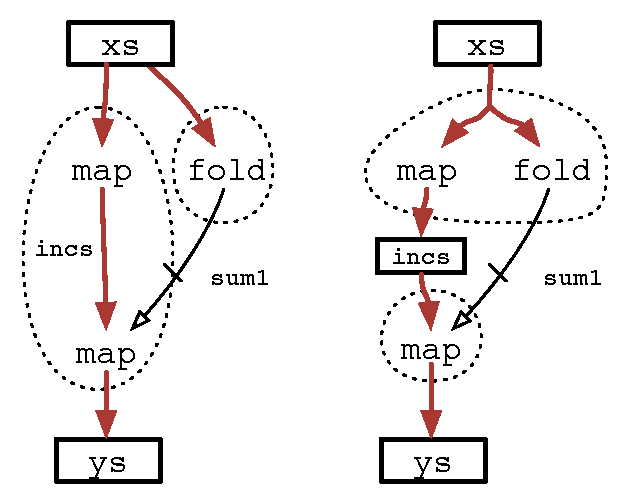
\includegraphics[scale=0.5]{figures/ex2-normalizeInc.pdf}
\end{center}
\caption{Possible clusterings for \texttt{normalizeInc}}
\label{f:normalizeInc}
\end{figure}


% -----------------------------------------------------------------------------
\section{Integer Linear Programming}
\label{s:ILP}
It is usually possible to cluster a program graph in multiple ways. For example, consider the following simple function:
\begin{code}
 normalizeInc :: Array Int -> Array Int
 normalizeInc xs
  = let incs = map  (+1)    us
        sum1 = fold (+) 0   us
        ys   = map  (/ sum) incs
    in  ys
\end{code}

Two possible clusterings are shown in Figure~\ref{f:normalizeInc}. One option is to compute @sum1@ first and fuse the computation of @incs@ and @ys@. Another option is to fuse the computation of @incs@ and @sum1@ into a single loop, then compute @ys@ separately. A third option (not shown) is to compute all results separately, and not perform any fusion. 

Which option is better? On current hardware we generally expect the cost of memory access to dominate runtime. The first clustering in Figure~\ref{f:normalizeInc} requires two reads from array @xs@ and one write to array @ys@. The second requires a single fused read from @xs@, one write to @incs@, a read back from @incs@ and a final write to @ys@. From the size constraints of the program we know that all intermediate arrays have the same size, so we expect the first clustering will peform better as it only needs three array accesses instead of four. 

For small programs such as @normalizeInc@ it is possible to naively enumerate all possible clusterings, select just those that are \emph{valid} with respect to fusion preventing edges, and chose the one that maximises a cost metric such as the number of array accesses needed. However, as the program size increases the number of possible clusterings becomes too large to naively enumerate. For example, Pouchet et al~\cite{pouchet2010combined} present a fusion system using the polyhedral model~\cite{pouchet2011polyhedral} and report that some simple numeric programs have over 40,000 possible clusterings, with one particular example having $10^{12}$. 

To deal with the combinatorial explosion in the number of potential clusterings, we instead use an Integer Linear Programming (ILP) formulation. ILP problems are defined as a set of variables, an objective linear function and a set of linear constraints. The integer linear solver finds an assignment to the variables that minimises the objective function, while satisfying all constraints. For the clustering problem we express our constraints regarding fusion preventing edges as linear constraints on the ILP variables, then use the objective function to encode our cost metric. This general approach was first fully described by Megiddo and Sarkar~\cite{megiddo1998optimal}, and our main contribution is to extend it to work with size changing operators such as @filter@. 


% -----------------------------------------------------------------------------
\subsection{Dependency Graphs}
A dependency graph represents the data dependencies of the program to be fused, and we use it as an intermediate stage when producing linear constraints for the ILP problem. The dependency graph contains enough information to determine the possible clusterings of the input program, while abstracting away from the exact operators used to compute each intermediate array. The rules for producing a dependency graphs are in Figure~\ref{f:DependencyGraph}.

Each binding in the source program becomes a node in the dependency graph. For each intermediate variable, we add a directed edge from the binding that produces a value to all bindings that consume it. Each edge is also marked as either \emph{fusible} or \emph{fusion preventing}. Fusion preventing edges are used when the producer must finish its execution before the consumer node can start. For example, a @fold@ operation must complete execution before it can produce the scalar value needed by its consumers. Conversely, the @map@ operation produces an output value for each value it consumes, so is marked as fusible. 

The @gather@ operation is a hybrid: it takes an indices array and an elements array, and for each element in the indices array returns the corresponding data element. This means that gather can be fused with the operation that produces its indices, but not the operation that produces its elements --- because those are accessed in a random-access manner. 

% Each node may simply be the name of its output binding (or bindings, in the case of @external@); as we require names to only be bound once, this is assured to be unique. Creating edges between these nodes is simply when one binding references an earlier one. The only complication is designating edges as \emph{fusible} or \emph{fusion-preventing}.

\begin{figure}
\begin{tabbing}
MMMMM       \= M  \= \kill
$nodes$     \> @:@ \> $\function \to V$              \\
$edges$     \> @:@ \> $\function \to E$              \\
$edge$      \> @:@ \> $\{bind\} \times bind \to E$   \\
$inedge$    \> @:@ \> $\{bind\} \times name \times name \to E$   \\
\\
$nodes(bs)$ \> $= \{(name(b), \iiter_{\Gamma,C}(b)) | b \in bs\}$       \\
\\
$edges(bs)$ \> $= \bigcup_{b \in bs}edge(bs, b)$    \\
\\
MM             \= M \= \kill
$edge(bs, out = @fold@~f~in)$ \\
    \> $=$    \> $\{inedge(bs,out,s) | s \in fv(f)\} \cup \{inedge(bs, out, in) \}$       \\
$edge(bs, out = @map@~f~in)$  \\
    \> $=$    \> $\{inedge(bs,out,s) | s \in fv(f)\} \cup \{inedge(bs, out, in) \}$       \\
$edge(bs, out = @filter@~f~in)$  \\
    \> $=$    \> $\{inedge(bs,out,s) | s \in fv(f)\} \cup \{inedge(bs, out, in) \}$       \\
$edge(bs, out = @gather@~data~indices)$  \\
    \> $=$    \> $\{(out,data, \fusionpreventing) \} \cup \{inedge(bs, out, indices) \}$       \\
$edge(bs, out = @cross@~a~b)$            \\
    \> $=$    \> $\{inedge(bs, out, a) \}           \cup      \{(out, b, \fusionpreventing) \}$ \\
$edge(bs, outs = @external@~ins)$  \\
    \> $=$    \> $\{(outs,i, \fusionpreventing) | i \in ins \}$ \\
\\
$inedge(bs,to,\from)$ \\
    \> $|$ \> $(\from = @fold@~f~s) \in bs$     \\
    \> $=$ \> $(to, \from, \fusionpreventing)$  \\
    \> $|$ \> $(outs = @external@ \ldots) \in bs     \wedge \from \in outs$     \\
    \> $=$ \> $(to, outs, \fusionpreventing)$  \\
    \> $|$ \> $otherwise$                      \\
    \> $=$ \> $(to, \from, \fusible)$
\end{tabbing}

\caption{Dependency Graphs from Programs}
\label{f:DependencyGraph}
\end{figure}


% -----------------------------------------------------------------------------
\subsection{ILP Variables}
After generating the dependency graph, the next step is to produce a set of linear constraints from this graph. The variables involved in these constraints are split into three groups:
\begin{tabbing}
M   \= MM \= MMMMMMM \= MM \= \kill
$x$   \> @:@  \> $node \times node$ \> $\to$ \> $\mathbb{B}$
\end{tabbing}
For each pair of nodes with indices $i$ and $j$ we use a boolean variable $x_{i,j}$ which indicates whether those two nodes are fused. We use $x_{i,j} = 0$ when the nodes are fused and $x_{i,j} = 1$ when they are not. Using $0$ for the fused case means that the objective function can be a weighted function of the $x_{i,j}$ variables, and minimizing it tends to increase the number of nodes that are fused. The values of these variables are used to construct the final clustering, such that $\forall i,j.\ x_{i,j} = 0 \iff cluster(i) = cluster(j)$.
\begin{tabbing}
M   \= MM \= MMMMMMM \= MM \= \kill
$\pi$ \> @:@  \> $node$             \> $\to$ \> $\mathbb{R}$
\end{tabbing}
The second group of variables is used to ensure that the clustering is acyclic. This means that for each node in the graph, the dependencies of that node can be executed before the node itself. For each node $i$, we associate a real $\pi_i$ such that every node $j$ that depends on $i$ we have $\pi_j > \pi_i$. Our linear constraints will ensure that if two nodes are fused into the same cluster then their $\pi$ values will be identical --- though nodes in different clusters can also have the same $\pi$ value. Here is an example of a cyclic clustering:
\begin{code}
  cycle xs  = let ys  = map (+1) xs     (C1)
                  sum = fold ys         (C2)
                  zs  = map (+sum) ys   (C1)
              in  zs
\end{code}
There is no fusion-preventing edge directly between the @xs@ and @zs@ bindings, but there is a fusion-preventing edge between @sum@ and @zs@. If the @xs@ and @zs@ bindings were in the same cluster @C1@ and @sum@ was in cluster @C2@, there would be a dependency cycle between @C1@ and @C2@, and neither could be executed before the other.
\begin{tabbing}
M   \= MM \= MMMMMMM \= MM \= \kill
$c$   \> @:@  \> $node$             \> $\to$ \> $\mathbb{B}$
\end{tabbing}
The final group of variables is used to help define the cost model encoded by the objective function. Each node is assigned a variable $c_i$ that indicates whether the array the associated binding produces is \emph{fully contracted}. When an array is fully contracted it means that all consumers of that array are fused into the same cluster, so we have $c_i = 0 \iff \forall (i',j) \in E.\ i = i' \implies x_{i,j} = 0$. In the final program, each successive element of a fully contracted array can be stored in a scalar register, rather than requiring an array register or memory storage. 


% -----------------------------------------------------------------------------
\subsection{Linear Constraints}
\label{s:LinearConstraints}
The constraints we place on the ILP variables are split into four groups: constraints that ensure the clustering is acyclic; constraints that encode fusion preventing edges; constraints on nodes with different iteration sizes, and constraints involving array contraction. 

% Before showing the optimised version with certain constraints removed (\S\ref{s:OptimisedConstraints}), this simpler, unoptimised version is shown. The only difference is that fewer constraints and variables are required in the optimised version, but both versions give the same clustering. This unoptimised version generates clustering constraints and variables for every pair of nodes, regardless of whether they may, in fact, be fused together. Later, we show that certain constraints and variables can be removed when there is a fusion-preventing edge between two nodes.


% -------------------------------------
\paragraph{Acyclic and precedence-preserving} The first group of constraints ensures that the clustering is acyclic:
\begin{tabbing}
MM  \= MMMx \= M \= MMM \= M \= MMMM \= \kill
    \> ~~~~~~~ $x_{i,j}$ \> $\le$ \> $\pi_j - \pi_i$ \> $\le$ \> $N \cdot x_{i,j}$ 
    \>             (with an edge from $i$ to $j$)            \\
    \> $-N \cdot  x_{i,j}$  \> $\le$ \> $\pi_j - \pi_i$ \> $\le$ \> $N \cdot x_{i,j}$ 
    \>             (with no edge from $i$ to $j$)
\end{tabbing}
As per Megiddo~\cite{megiddo1998optimal} the form of these constraints is determined by whether there is an dependency between nodes $i$ and $j$. The $N$ value is set to the total number of nodes in the graph.

If there is an edge from node $i$ to $j$ we use the first constraint form shown above. If the two nodes are fused into the same cluster then we have $x_{i,j} = 0$. In this case the constraint simplifies to $0 \le \pi_j - \pi_i \le 0$, which forces $\pi_i = \pi_j$. If the two nodes are in \emph{different} clusters then the constraint instead simplifies to $1 \le \pi_j - \pi_i \le N$. This means that the difference between the two $\pi$s must be at least 1, and less than $N$. Since there are $N$ nodes, the maximum difference between any two $\pi$s would be at most $N$, so the upper bound of $N$ is large enough to be safely ignored. This means the constraint can roughly be translated to $\pi_i < \pi_j$, which enforces the acyclicity constraint.

If instead there is no edge from node $i$ to $j$ then we use the second constraint form above. As before, if the two nodes are fused into the same cluster then we have $x_{i,j} = 0$, which forces $\pi_i = \pi_j$. If the nodes are in different clusters then the constraint simplifies to $-N \le \pi_j - \pi_i \le N$, which effectively puts no constraint on the $\pi$ values.


% -------------------------------------
\paragraph{Fusion-preventing edges} As per Megiddo~\cite{megiddo1998optimal}, if there is a fusion preventing edge between two nodes we add a constraint to ensure the nodes will be placed in different clusters.
\begin{tabbing}
MMM     \= MMM \= M  \= MMM \= M \= MMM \= \kill
        \> $x_{i,j}$ \> $=$ \> $1$ \>   \> \\
        \> (for fusion-preventing edges from $i$ to $j$) 
\end{tabbing}
When combined with the precedence-preserving constraints earlier, setting $x_{i,j} = 1$ also forces $\pi_i < \pi_j$. 


% -------------------------------------
\paragraph{Fusion between different iteration sizes} This group of constraints restricts which nodes can be placed in the same cluster based on their iteration size. The group has three parts. 
Firstly, either of the two nodes connected by an edge have an unknown ($\bot$) iteration size then they cannot be fused and we set $x_{i,j} = 1$:
\begin{tabbing}
MMM     \= MMM \= M \= MMM \= M \= MMM \= \kill
        \> $x_{i,j}$   \> $=$   \> $1$          \>       \>     \\
        \> (if $\iiter_{\Gamma,C}(i) = \bot 
                ~\vee~ \iiter_{\Gamma,C}(j) = \bot$)
\end{tabbing}
Secondly, if the two nodes have different iteration sizes and no common parent then they also cannot be fused and we set $x_{i,j} = 1$:
\begin{tabbing}
MMM     \= MMM \= M \= MMM \= M \= MMM \= \kill
        \> $x_{i,j}$   \> $=$   \> $1$          \>       \>     \\
        \> (if $\iiter_{\Gamma,C}(i) \not= \iiter_{\Gamma,C}(j) 
                ~\wedge~ parents(i,j) = \emptyset$)
\end{tabbing}
Finally, if the two nodes had different iteration sizes but \emph{do} have parent transducers of the same size, then the two nodes can be fused if they are fused with their respective parents, and the parents themselves are fused:
\begin{tabbing}
MMM     \= MMM \= M \= MMM \= M \= MMM \= \kill
        \> $x_{a,A}$   \> $\le$ \> $x_{a,b}$    \>       \>     \\
        \> $x_{b,B}$   \> $\le$ \> $x_{a,b}$    \>       \>     \\
        \> $x_{A,B}$   \> $\le$ \> $x_{a,b}$    \>       \>     \\
        \> (if $\iiter_{\Gamma,C}(a) \not= \iiter_{\Gamma,C}(b) 
                ~\wedge~ parents(a,b) = \{(A,B)\}$)
\end{tabbing}
This last part is the main difference to existing ILP solutions: we allow nodes with different iteration sizes to be fused when their parent transducers are fused. The actual constraints encode a ``no more fused than'' relationship. For example $x_{a,A} \le x_{a,b}$ means that nodes $a$ and $b$ can be no more fused than nodes $a$ and $A$. 

As a simple example, consider fusing an operation on filtered data with its generating filter:
\begin{code}
    sum1 = fold (+) 0  xs
    gts  = filter (>0) xs
    sum2 = fold (+) 0  gts
\end{code}
Here $sum1$ and $sum2$ have different iteration sizes and we have that $parents(sum1, sum2) = \{(sum1, gts)\}$. This means that $sum1$ and $sum2$ may only be fused if $sum1$ is fused with $sum1$ (trivial), $sum2$ is fused with $gts$, and $sum1$ is fused with $gts$.

% Here, $parents(gts,sum2) = \{gts, gts\}$. This generates spurious, but still valid, constraints that $gts$ must be fused with $gts$ and $gts$ must be fused with $sum2$, in order for $gts$ and $sum2$ to be fused together. While these constraints are unnecessary in this case, they are harmless.

% While it may seem like these constraints should be implied by transitivity of clustering, all clustering variables are used for the objective function.


% -------------------------------------
\paragraph{Array contraction} The final group of constraints gives meaning to the $c$ variables that we use to represent whether an array is fully contracted:
\begin{tabbing}
MMM     \= MMM \= M \= MMM \= M \= MMM \= \kill
        \> $x_{i,j}$    \> $\le$ \> $c_i$  \> \> \\
        \> (for all edges from i)
\end{tabbing}
Recall that an array is fully contracted when all of the consumers are fused with the nodes that produces it, which means that the array does not need to be fully materialized in memory. As per Darte's work on array contraction~\cite{darte2002contraction}, we define a variable $c_i$ for each array, and the constraint above ensures that $c_i = 0$ only if $\forall (i',j) \in E.\ i = i' \implies x_{i,j} = 0$. By minimizing $c_i$ in the objective function, we favor solutions that reduce the number of intermediate arrays.


% -----------------------------------------------------------------------------
\subsection{Objective Function}
\label{s:ObjectiveFunction}
The objective function defines the cost model of the program, and the ILP solver will find the clustering that minimizes this function while satisfying the constraints defined in the previous section. The cost model we use in this paper has three components:
\begin{itemize}
\item
the number of array reads and writes --- an abstraction of the amount of memory bandwidth needed by the program; 
\item
the number of intermediate arrays --- an abstraction of the amount of intermediate memory needed; 
\item
the number of distinct clusters --- an abstraction of the cost of loop management instructions, which maintain loop counters and the like.
\end{itemize}
The three components of the cost model are a heuristic abstraction of the true cost of executing the program on current hardware. They are ranked in order of importance --- so we prefer to minimize the number of array reads and writes over the number of intermediate arrays, and to minimize the number of intermediate arrays over the number of clusters. However, minimizing one component does not necessarily minimize any other. For example, as the fused program executes multiple array operations at the same time, in some cases the clustering that requires the least number of array reads and writes uses more intermediate arrays than strictly necessary.

We encode the ordering of the components of the cost model as different weights in the objective function. First, note that if the program graph contains $N$ combinators (nodes) then there are at most $N$ opportunities for fusion. We then encode the relative cost of loop overhead as weight $1$, the cost of an intermediate array as weight $N$, and the cost of an array read or write as weight $N^2$. This ensures that no amount of loop overhead reduction can outweigh the benefit of removing an intermediate array, and likewise no number of removed intermediate arrays can outweigh a reduction in the number of array reads or writes. The integer linear program including the objective function is as follows:
\begin{tabbing}
MMMMM   \= MMMM \= M \= \kill
Minimise   \>     \> $\Sigma_{(i,j) \in E} W_{i,j} \cdot x_{i,j}$   
\\         \> \> \> (memory traffic and loop overhead)              
\\         \> $+$ \> $\Sigma_{i \in V} N \cdot c_i$                  
\\         \> \> \> (removing intermediate arrays)         
\\ Subject to \> \ldots ~ constraints from \S\ref{s:LinearConstraints} ~ \ldots 
\\ Where      \>                                       
\\         \> $W_{i,j} = N^2$ \> $~|$ \> $(i,j) \in E $         
\\         \> \> \> (fusing $i$ and $j$ will reduce memory traffic)         
\\         \> $W_{i,j} = N^2$ \> $~|$ \> $\exists k. (k,i) \in E \wedge (k,j) \in E $     
\\         \> \> \> ($i$ and $j$ share an input array)
\\         \> $W_{i,j} = 1$   \> $~|$ \> $@otherwise@$
\\         \> \> \> (the only benefit is loop overhead)
\\         \> $N = |V|$
\end{tabbing}

% However, these benefits cannot be considered in isolation; for example, fusing two loops to reduce loop overhead may remove potential fusion opportunities that reduce memory traffic. When operating on large arrays that do not fit in cache, memory traffic dominates execution time. An excessive number of intermediate arrays can also cause issues if all are live in memory at once, potentially leading to \emph{thrashing}. The benefits of removing loop overhead are least of all; it should be performed if possible, but must never remove opportunities for other fusion.



% -----------------------------------------------------------------------------
\subsection{Fusion-preventing Path Optimisation}
\label{s:OptimisedConstraints}
The integer linear program defined in the previous section includes more constraints than strictly necessary to define the valid clusterings. If two nodes have a path between them which includes a fusion preventing edge, then we know up front that they must be placed in different clusters. The following function $possible(a,b)$ determines whether there is any possibility that the two nodes $a$ and $b$ can be fused. Similarly the function $possible'(a, b)$ checks whether there is any possibility that the parents of $a$ and $b$ may be fused.

\newpage

\begin{tabbing}
MMMM \= M \=     \= MMMMMMMMMMMM    \=  \kill
$possible$ \> $:$     \> $name \times name \to \mathbb{B}$      \\
MM        \= M    \= \kill
$possible(a,b)$ \\
    \>$=$  \>$\forall p \in path(a,b) \cup path(b,a).\ \fusionpreventing \not\in p$
\\[1ex]
MMMM \= M \=     \= MMMMMMMMMMMM    \=  \kill
$possible'$     \> $:$ \> $name \times name \to \mathbb{B}$      \\
MM        \= M    \= \kill
$possible'(a,b)$ \\
    \>$=$   \>$\exists A, B.\  parents(a,b) = \{A,B\} \wedge possible(a,b)$ \\
    \>$\wedge$ \> $possible(A,a) \wedge possible(B,b) \wedge possible(A,B)$
\end{tabbing}
With $possible$ and $possible'$ defined, we refine our formulation to only generate constraints between two nodes if there is a chance they may be fused together. Doing this reduces the total number of constraints, and makes the job of the ILP solver easier. The final formulation of the integer linear program follows.

\begin{tabbing}
MMMMM   \= MMMM \= M \= MMMM \= M \= MMMM \= \kill
Minimise   \> $\Sigma_{(i,j) \in E} W_{i,j} \cdot x_{i,j} + \Sigma_{i \in V} N \cdot c_i$  \\
           \> (if $possible(i,j)$)         \\
Subject to \\
           \> $-N \cdot x_{i,j}$ \> $\le$ \> $\pi_j - \pi_i$ \> $\le$ \> $N \cdot x_{i,j}$ \\
           \> (if $possible(i,j) \wedge (i,j) \not\in E \wedge (j,i) \not\in E$)            
\\[1ex]
           \>    $x_{i,j}$ \> $\le$ \> $\pi_j - \pi_i$ \> $\le$ \> $N \cdot x_{i,j}$ \\
           \> (if $possible(i,j) \wedge (i,j,\fusible) \in E$)     
\\[1ex]
           \>             \>       \> $\pi_i < \pi_j$ \>       \>            \\
           \> (if $(i,j,\fusionpreventing) \in E$)    
\\[1ex]
           \> $x_{i,j}$    \> $\le$ \> $c_i$           \>       \>            \\
           \> (if $(i,j, \fusible) \in E$) \\
           \> $c_{i }$    \> $ = $ \> $ 1 $           \>       \>            \\
           \> (if $(i,j, \fusionpreventing) \in E$) \\
\\[1ex]
           \> $x_{i,j}$    \> $=$   \> $1$             \>       \>            \\
           \> (if $\bot \in \{\iiter_{\Gamma,C}(i), \iiter_{\Gamma,C}(j)\}$)  
\\[1ex]
           \> $x_{i',i}$   \> $\le$ \> $x_{i,j}$        \>       \>            \\
           \> $x_{j',j}$   \> $\le$ \> $x_{i,j}$        \>       \>            \\
           \> $x_{i',j'}$   \> $\le$ \> $x_{i,j}$        \>       \>            \\
           \> (if $\iiter_{\Gamma,C}(i) \not= \iiter_{\Gamma,C}(j) \wedge possible'(i,j)$ \\
           \> \> $\wedge~parents(i,j) = \{(i',j')\}$) 
\\[1ex]
           \> $x_{i,j}$    \> $=$   \> $1$             \>       \>            \\
           \> (if $\iiter_{\Gamma,C}(i) \not= \iiter_{\Gamma,C}(j) \wedge \neg possible'(i,j)$) \\
MMMMM   \= MMMM \= M \= \kill
Where      \>                                       \\
           \> $W_{ij} = N^2$ \> $~|$ \> $(i,j) \in E $         \\
           \> \> \> (fusing $i$ and $j$ will reduce memory traffic)         \\
           \> $W_{ij} = N^2$ \> $~|$ \> $\exists k. (k,i) \in E \wedge (k,j) \in E $     \\
           \> \> \> ($i$ and $j$ share an input array)                                         \\
           \> $W_{ij} = 1$   \> $~|$ \> $@otherwise@$                                                  \\
           \> \> \> (the only benefit is loop overhead)                                        
\\[1ex]
           \> $N = |V|$
\end{tabbing}

% % !!!!!!!!!!!!!!!!!!!!!!!
% I commented the \input out in section/04-ILP.tex

\subsection{Proof}
To prove correctness of our linear program formulation, we need to prove two different things.
Firstly, the formulation's constraints must always be satisfiable; that is, there must exist a variable assignment that satisfies all constraints.
This is rather simple to show, but guarantees that the linear program will always give an answer.
The next thing to show is that any produced clustering is legal: if a variable assignment satisfies the constraints, then it is a valid and legal clustering.
This means that, not only do we get \emph{an} answer, we also get the \emph{right} answer.

%!TEX root = ../Main.tex
\subsubsection{Satisfiability}
For any program $p$, there exists a trivial clustering with no fusion at all.
We can use this as the variable assignment of $ilp(p)$.
For each pair of nodes $m,n \in p$, $x_{mn} = 1$ --- no fusion is possible.
For the $\pi$ variables, we must find a topographical ordering of the nodes in $p$, which is simple since we are assured it is a dag.

\TODO{Now, prove that this assignment actually satisfies the constraints.}


\subsubsection{Soundness}
For any program $p$ and variable asignment $v$, if $v$ satisfies the constraints for $ilp(p)$, the clustering denoted by $x_{ij}$ in $v$ is legal.

For a clustering to be legal, it must satisfy three constraints:
\begin{description}
\item[Acyclic]
after merging nodes of same cluster together, the resulting graph must be a dag
\item[Precedence preserving]
if there is an edge between two nodes $i$ and $j$, and they are not merged together, then we require $\pi_j > \pi_i$
\item[Fusion preventing]
likewise, if there is a fusion-preventing edge between two nodes $i$ and $j$, then we require $\pi_j > \pi_i$, which implies that they are not merged together
\item[Type constraint]
if two nodes $i$ and $j$ are in the same cluster, then $\tau_i = \tau_j$, or if $\tau_i$ is a subtype of $\tau_j$ (or $\tau_j$ is a subtype of $\tau_i$), then the \emph{generator} for $\tau_i$ (or $\tau_j$) must also be in the same cluster as $i$ and $j$.
    \\
    \TODO Actually, let us say $x_{ij} = 0 \implies check_{ij}$

\end{description}
where
\begin{tabbing}
MMMMM      \= M \= MMMMMMM \= MM \= \kill
$check$ \> @::@  \> $array \times array$ \> $\to$ \> $\mathbb{B}$ \\
MMMMM      \= M \= MMMMMM \= MM \= \kill
$check(i, j)$     \> $|$ \> $tau_i = tau_j$ \> $=$ \> $x_{i,j} = 0$                        \\
$check(i, j)$     \> $|$ \> $i' \in gen(i) $ \> $=$ \> $x_{i',j} = 0 \wedge x_{i,i'} = 0 \wedge check(i', j)$                        \\
$check(i, j)$     \> $|$ \> $j' \in gen(j) $ \> $=$ \> $x_{i,j'} = 0 \wedge x_{j,j'} = 0 \wedge check(i, j')$                        \\
$check(i, j)$     \> $|$ \> $tau_i \not= tau_j$\> $=$ \> $\bot$
\end{tabbing}









\section{Related work}

\subsection{Haskell short-cut fusion}
Existing fusion systems for Haskell such as stream fusion\cite{coutts2007streamfusion}, tend to cleverly reuse compiler optimisations such as inlining and rewrite rules, to fuse combinators without having to modify the compiler itself.
This approach has the advantage of simplicity, but is inherently limited in the amount of fusion it can perform.

Consider the following @filterMax@ function, where each element in the input array is incremented, then the maximum is found, and the array is filtered to those greater than zero.
In this case, the result of the map @vs'@ cannot be inlined into both occurences without duplicating work, so no fusion can be performed.
This has the effect of performing three loops instead of one, with two arrays instead of one.

\begin{code}
filterMax vs =
 let vs' = map    (+1)  vs
     m   = fold   max 0 vs'
     flt = filter (>0)  vs'
\end{code}

\subsection{Integer linear programming in imperative languages}
The idea of using integer linear programming to find optimal fusion clusterings is not new, and has been discussed for imperative languages before.
These methods first construct a \emph{loop dependence graph} (LDG) from a given program, and then use this graph to create the integer linear program.
The LDG has nodes for each loop in the program, and edges between loops are dependencies.
Edges may be fusible, or fusion-preventing, in which case the two nodes may not be merged together.

Talk about the simple formulation by Darte\cite{darte2002new}.
Has an integer variable for each node, denoting the number of the cluster it's in.
Also includes a binary variable for each node, which is whether the node is fused with all its successors - in which case no array would be required, and an integer variable which is the maximum of all cluster numbers.
The objective function is to maximise the number of nodes that are completely fused, requiring no arrays, and minimise the maximum cluster number, which in turn minimises the number of clusters.
It doesn't require many constraints and is easy to implement, but doesn't work as well when there are loops of different sizes.
As loops of different sizes cannot be fused together, a simple method is to introduce an ordering on the sizes, and then extract loops of the same cluster number in order of size.
The problem here is that the objective function uses the maximum cluster number to minimise the number of loops, but this alone is no longer sufficient when there are multiple sizes. Explain why.


The formulation by Megiddo\cite{megiddo1997optimal} supports different sized loops, and is therefore more relevant for our purposes.
For every pair of nodes $i,j$ in the LDG, a variable $x_{ij}$ is created, which denotes whether $i$ and $j$ are fused together.
Slightly awkwardly, but for simplicity of other constraints, $x_{ij} = 0$ if the two nodes are fused together.
If there is a fusion preventing edge between $i$ and $j$, then $x_{ij}$ is constrained to be $1$ - that is, no fusion is possible.
This alone is not enough to guarantee a valid clustering.
To constrain the solution to acyclic and precedence preserving clusterings, a variable $\pi_i$ is added for each node $i$.
Constraints are added that require two nodes $i,j$ to have $\pi_i = \pi_j$ if $x_{ij} = 0$, and otherwise $\pi_i > \pi_j$ if $i$ is after $j$.
For each pair of nodes, a weight constant $w_{ij}$ is given, and the objective function is to minimise $\Sigma_{ij} w_{ij} x_{ij}$, which has the effect of maximally fusing nodes, according to their weights.

The difference to our combinator-based approach is that with combinators we retain more information about the meaning of the program.



\section{Motivating programs}
\ben{Use the larger programs as benchmarks, or as running examples. We only need small, simple programs to demonstrate how the algorithm works.}


\subsection{Quickselect}
We can't quite do @quickselect@, sadly; it requires @head@.
\begin{code}
select :: Vec a -> Int -> a
select xs k
 | length xs > 0
 = let p    = head xs 
       xslt = filter  (<p) xs
       xsge = filter (>=p) xs
   in  if     length xslt > k
       then   select xsge (k - length xslt)
       else   select xslt  k
 | length xs == 1
 = head xs
 | length xs == 0
 = error "Empty array!"

median :: Vec a -> a
median xs
 = select xs (length xs `div` 2)
\end{code}

\subsection{Closest pairs}
Closest pairs makes use of fast-ish @median@ to ensure balanced division of work.
\begin{code}
closest :: Vec Pt -> (Pt,Pt)
closest pts
 | length pts < 250
 = naive pts
 | otherwise
 = divide pts

divide :: Vec Pt -> (Pt,Pt)
divide pts
 = let p      = median pts
       aboves = filter (above p) pts
       belows = filter (below p) pts
       above' = closest aboves
       below' = closest belows

       border = min (distance above') (distance below')

       aboveB = filter (above (p - border)) pts
       belowB = filter (below (p + border)) pts

       cs     = cross aboveB belowB
       bord   = minBy distance cs
   in  above' `minDist` below' `minDist` bord


naive :: Vec Pt -> (Pt,Pt)
naive pts
 = let c = cross pts pts
   in  minBy distance c

minBy :: Ord b => (a -> b) -> Vec a -> a
minBy f xs
 = fold (min . f...) ... xs
\end{code}

Let's translate @divide@ to a program in CNF.
\begin{code}
divide :: Vec Pt -> (Pt,Pt)
divide pts
 = let p      = external pts

       aboves = filter (... p) pts          -- A
       belows = filter (... p) pts          -- A

       above' = external aboves
       below' = external belows
       border = external above' below'

       aboveB = filter (... p border) pts   -- C
       belowB = filter (... p border) pts   -- B

       cs     = cross  aboveB belowB        -- C
       bord   = fold   (...) cs             -- C

       min'   = external above' below' bord
   in  min'
\end{code}
where @A@, @B@ and @C@ are distinct clusters.

What happens if we do this using stream fusion?
\begin{code}
divide :: Vec Pt -> (Pt,Pt)
divide pts
 = let p      = external pts

       aboves = filter (... p) pts          -- A
       belows = filter (... p) pts          -- B

       above' = external aboves
       below' = external belows
       border = external above' below'


       aboveB = filter (... p border) pts   -- D
       belowB = filter (... p border) pts   -- C

       cs     = cross  aboveB belowB        -- D
       bord   = fold   (...) cs             -- D

       min'   = external above' below' bord
   in  min'
\end{code}
So, we have four clusters instead of three, and the same number of manifest arrays. Not particularly impressive.

\subsection{Quickhull}
Is Quickhull any better? Seems like it's just one cluster; @filterMax@. And we don't have append (@++@), anyway.
\begin{code}
quickhull :: Vec Pt -> Vec Pt
quickhull pts
 = let top  = fold getTop pts
       bot  = fold getBot pts
       tops = hull (top,bot) pts
       bots = hull (bot,top) pts
   in  tops ++ bots

hull :: (Pt,Pt) -> Vec Pt -> Vec Pt
hull line@(l,r) pts
 = let pts' = filter (above   line) pts
       ma   = fold   (maxFrom line) pts'
       hl   = hull   (l, ma)        as
       hr   = hull   (ma, r)        as
   in  hl  ++ hr
\end{code}
Yep. @hull@ is pretty boring.

Something with a \emph{fold}, and then filtering or mapping based on that fold would be good.
Or something with
\begin{code}
let xs' = filter f    xs
    i   = fold   g    xs'
    xs''= map   (h i) xs'
\end{code}
would be really good.

FFT - not really.

\subsection{QuadTree}
\begin{code}
bounds pts
 = let x1 = fold minX pts
       y1 = fold minY pts
       x2 = fold maxX pts
       y2 = fold maxY pts
   in ((x1,y1), (x2,y2))

%splitbox ((x1,y1), (x2,y2))
% = let xm = mid x1 x2
%       ym = mid y1 y2
%   in ( ((x1, y1), (xm, ym))
%      , ((x1, ym), (xm, y2))
%      , ((xm, y1), (x2, ym))
%      , ((xm, ym), (x2, y2)))
%
quadtree pts
 = go (bounds pts)
 where
  go bounds pts
   | length pts > 0
   = let (b1,b2,b3,b4) = splitbox bounds
         pts1  = filter (inbox b1) pts
         pts2  = filter (inbox b2) pts
         pts3  = filter (inbox b3) pts
         pts4  = filter (inbox b4) pts
         tree1 = go b1 pts1
         tree2 = go b2 pts2
         tree3 = go b3 pts3
         tree4 = go b4 pts4
      in Tree tree1 tree2 tree3 tree4
   | otherwise
   = Empty
\end{code}
It's easy to see that @bounds@ should only require one loop, but stream fusion requires four, as there is no inlining that can occur.
The same is true of @go@ in @quadtree@. Our implementation only requires one loop for each of these.

\section{Conclusion}

\section*{Acknowledgements}
Many thanks are due to
Robert Clifton-Everest,
Kai Engelhardt,
Bill Kroon,
Frederik Madsen,
Abdallah Saffidine,
and Jingling Xue
for enlightening discussions relating to this work.

\bibliographystyle{plain}
\bibliography{Main}

\end{document}


